\chapter{Volar con PX4 o con ArduPilot}
\label{cap:pilotos}

\begin{enpocas}
Cómo se conecta la misión a cada piloto automático, cómo corre la red neuronal en cada uno, y la estación
de tierra (MAVProxy) con sus ventanas y su mapa.
\end{enpocas}

\section{Con PX4 (\texorpdfstring{\texttt{piloto:=px4}}{piloto:=px4}, por omisión)}

El \emph{launch} abre Gazebo con el bosque (sin la configuración de PX4), arranca el agente uXRCE-DDS en
el puerto 8888 y PX4 SITL (\cod{px4_sitl_neural}, \emph{airframe} 4099) conectado a ese Gazebo
(\cod{PX4_GZ_STANDALONE}). La misión habla con PX4 por ROS~2: lee \cod{/fmu/out/vehicle_odometry} y
\cod{/fmu/out/vehicle_status_v1}, y publica \cod{/fmu/in/trajectory_setpoint},
\cod{/fmu/in/offboard_control_mode} y comandos (\cod{/fmu/in/vehicle_command}). La red corre dentro de
PX4, en \cod{mc_nn_control}.

\section{Con ArduPilot (\texorpdfstring{\texttt{piloto:=ardupilot}}{piloto:=ardupilot})}

\begin{itemize}
  \item ArduCopter 4.7.2 se lanza directo (sin MAVProxy ni ventana propia) con los parámetros de
        \cod{config/ardupilot/x500.parm}, el \emph{home} en el origen del mundo y el vehículo dentro del
        mundo a 1~kHz.
  \item \cod{mision_ardupilot} (una subclase de la misión) se conecta por TCP 5760 con MAVLink, vuela en
        GUIDED con \cod{SET_POSITION_TARGET_LOCAL_NED} y publica el estimado del EKF de ArduPilot en
        \cod{/fmu/out/vehicle_odometry}, para que el localizador sea exactamente el mismo.
  \item Con \cod{controlador:=red}, la red corre en \cod{controlador_red} (ROS~2 + gz-transport,
        $\sim$330~Hz, 70~µs por paso) con el estado de Gazebo y manda
        $\omega_i = 1000\sqrt{(a_i+1)/2}$~rad/s. La misión publica ``red'' en \cod{/x500/controlador} y
        \cod{SelectorMotores} deja pasar esos comandos; ArduPilot sigue estimando, recibe las mismas
        consignas y recupera los motores para aterrizar, o si la red deja de publicar 50~ms.
\end{itemize}

\section{La estación de tierra: MAVProxy}

Con GUI, el \emph{launch} abre MAVProxy en su propia terminal, con consola, mapa y el módulo
\cod{mision.mavproxy_trayectoria}, conectado a PX4 por UDP 14550 o a ArduPilot por TCP 5762;
\cod{ventanas_sitl} acomoda las ventanas (terminal y consola a la izquierda, Gazebo al centro, mapa a la
derecha). El mapa dibuja la ruta planeada, la trayectoria recorrida y cada persona avisada.

\begin{figure}[H]
\centering
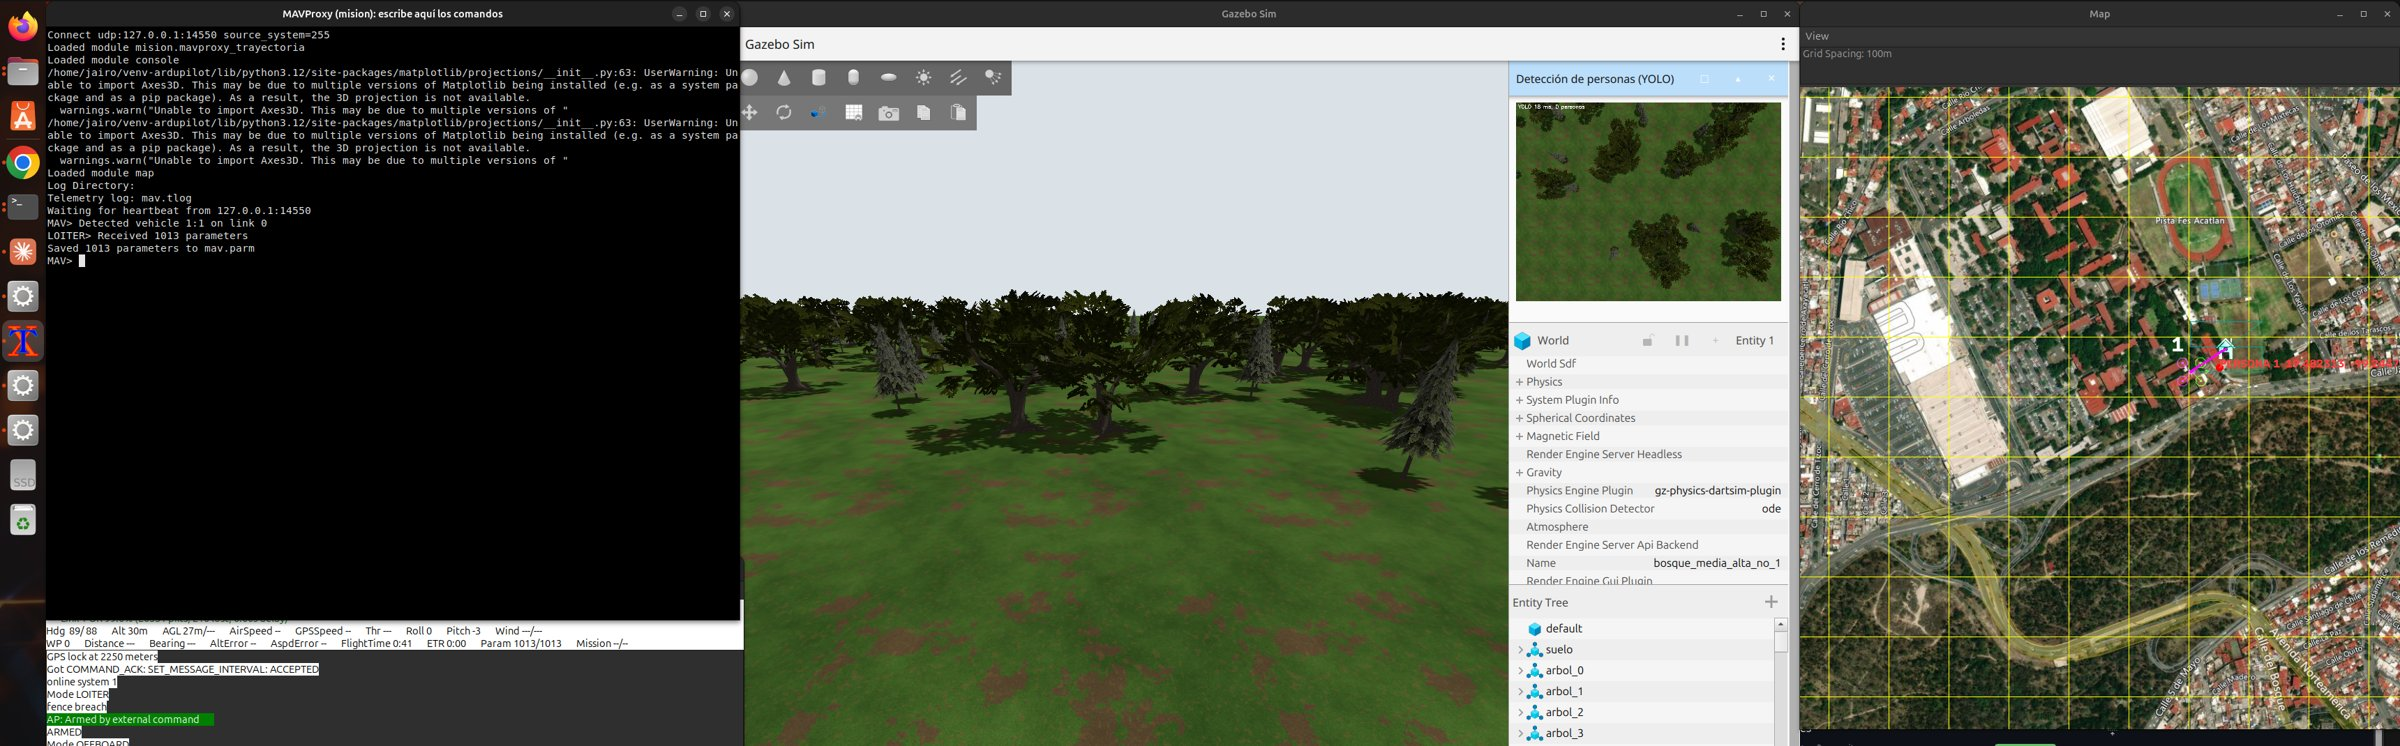
\includegraphics[width=\textwidth]{pantalla_mavproxy.jpg}
\caption{MAVProxy conectado a PX4: la terminal (con el prompt para escribir comandos), la consola, Gazebo
y el mapa.}
\end{figure}

\begin{longtable}{>{\raggedright\arraybackslash}p{5cm}p{10cm}}
\toprule
\textbf{Comando en MAVProxy} & \textbf{Efecto} \\ \midrule \endhead
\cod{mode LOITER} / \cod{mode RTL} / \cod{mode LAND} & detenerse, regresar al despegue, aterrizar \\
\cod{arm throttle} / \cod{disarm} & armar / desarmar \\
\cod{param show MPC_*} & ver parámetros (PX4) \\
\cod{trayectoria borrar|ocultar|mostrar} & dibujo de la trayectoria en el mapa \\
\bottomrule
\end{longtable}

\begin{aviso}
Si tomas el control desde MAVProxy, la misión sigue mandando consignas de offboard (PX4) o GUIDED
(ArduPilot). Al regresar a ese modo el dron retoma la búsqueda.
\end{aviso}

\section{Una simulación a la vez}

El \emph{launch} usa \cod{/clock}, \cod{/camera} y el puerto 8888 del agente. Para correr otra
simulación al mismo tiempo (por ejemplo, otra de ROS en la misma computadora), lánzala en otra partición
de Gazebo y otro dominio de ROS:
\begin{lstlisting}[style=bash]
GZ_PARTITION=busqueda ROS_DOMAIN_ID=7 ros2 launch mision simulacion.launch.py
\end{lstlisting}
Dos PX4 al mismo tiempo no se puede sin cambiar puertos: por eso la campaña corre los vuelos uno por uno.
